\section{Microcontrollers}

\paragraph*{Microprocessors}
Microprocessors serve as the backbone of general-purpose computers and are utilized in a wide range of applications, from desktops to servers and supercomputers. 
Designed to deliver high to very high computational power, they require significant external memory resources to operate effectively. 
Characterized by complex multi-core architectures, microprocessors typically boast clock speeds ranging from 2 to 5 GHz. However, they come with high costs, often falling between €100 and €5000, and exhibit substantial power consumption, ranging from 50 to 1500 watts. 
Additionally, microprocessors tend to have large form factors and limited interaction capabilities with their external environments.
\begin{figure}[H]
    \centering
    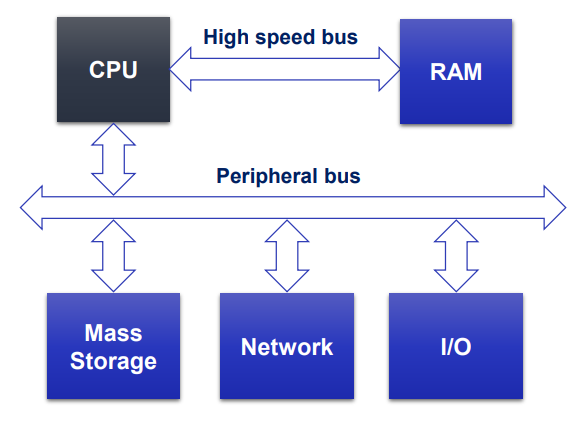
\includegraphics[width=0.75\linewidth]{images/micpro.png}
    \caption{Microprocessors structure}
\end{figure}

\paragraph*{Microcontrollers}
In contrast, microcontrollers are specifically designed for dedicated or embedded applications, where they perform targeted computational tasks. 
These devices incorporate small, integrated memory solutions, making them ideal for various applications, including home appliances and automotive systems.
Microcontrollers feature simpler architectures, typically employing 8, 16, or 32-bit designs with small pipelines. 
Their clock speeds generally range from 8 to 160 MHz, allowing for efficient processing of specific tasks. 
Priced affordably between €0.5 and €10, microcontrollers are designed with low power consumption in mind, often consuming between 0.1 and 300 milliwatts. 
Their compact form factor enables easy integration into diverse environments, where they are engineered to interact closely with external elements.
\begin{figure}[H]
    \centering
    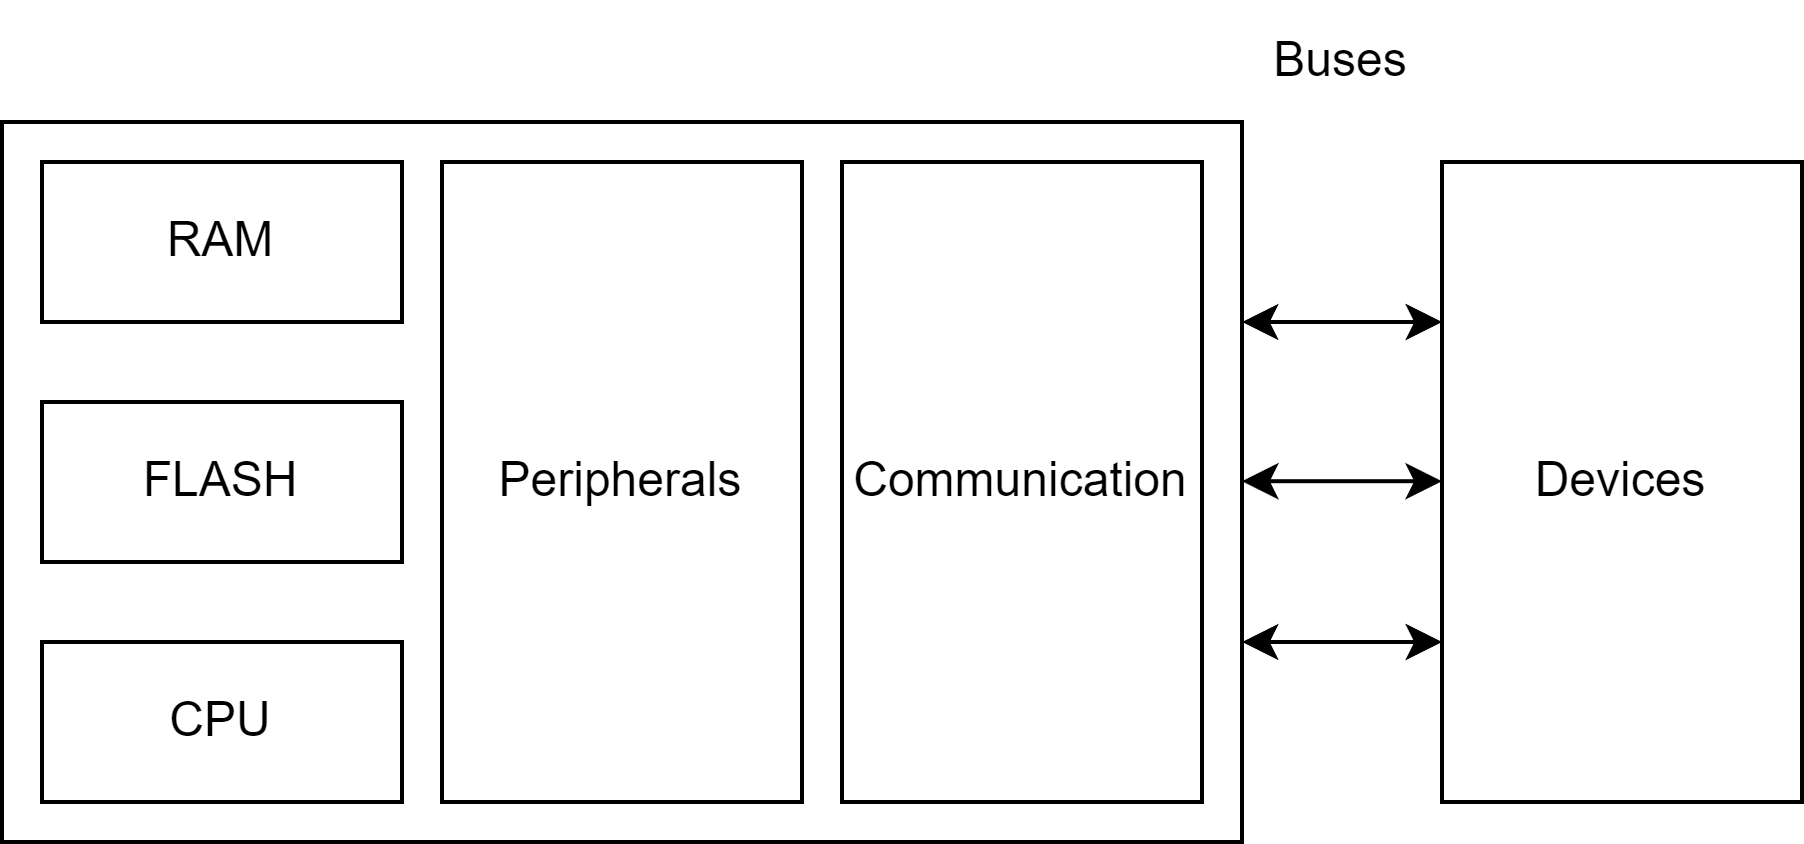
\includegraphics[width=0.75\linewidth]{images/miccon.png}
    \caption{Microcontrollers structure}
\end{figure}

\subsection{Clock}
The clock is a fundamental component that synchronizes all subsystems, including the core, memories, and peripherals. 
In typical systems, two primary types of clocks are utilized: the main clock and the real-time clock (RTC). 
The main clock is responsible for driving the core, memories, and peripherals, operating within a frequency range of 2 MHz to 144 MHz. 
On the other hand, the RTC is primarily used for timekeeping and is often employed in low-power modes, typically operating at a frequency of 32,768 Hz.

Clock signals can originate from various sources. 
Internal oscillators, while convenient, tend to be imprecise due to drift caused by temperature fluctuations and significant process variability. 
To mitigate these issues, the frequency generated by an internal oscillator is adjusted through a Digital Phase-Locked Loop (DPLL), and it is often paired with an external crystal to enhance stability. 
In contrast, external oscillators provide higher accuracy as they operate independently of the microcontroller. 
Similar to internal oscillators, their frequencies can also be adjusted with a DPLL and are frequently used in conjunction with an external crystal.

Moreover, several internal secondary sources contribute to clock management. 
The main clock can be multiplied or divided by dedicated clock generation and distribution logic, which enables various clock feeds to supply different domains. 
Each clock domain can be individually controlled, allowing for regulation and gating tailored to specific needs.

A clock domain is defined as a group of elements that are powered by the same clock. 
The core domain includes components such as the CPU, RAM, FLASH memory, and timers, while the analog domain encompasses analog-to-digital converters (ADCs), digital-to-analog converters (DACs), and comparators. 
The bus domain incorporates interfaces like SPI, UART, and I2C, and specific domains are dedicated to protocols such as Ethernet and USB. 
The ability to configure interconnects among these domains ensures flexible clock distribution, which is crucial for adapting to the varying requirements of different applications.

Key characteristics of effective clock management include maintaining low drift over time and temperature, particularly for specific peripherals like watchdog timers. 
Typically, drift values are around 1\%. 
Accuracy is another critical factor, especially for precise time measurement, which should fall within a range of 5 to 50 parts per million (ppm). 
Higher accuracy can be achieved through specialized devices or periodic resynchronization. Lastly, power consumption is an important consideration; techniques such as frequency scaling and clock gating are employed to save power during idle periods, contributing to the overall energy efficiency of the system.

\paragraph*{Real-Time Clock}
The real-time clock (RTC) serves two primary functions: calendar timekeeping and generating periodic alarms.
It is designed for high accuracy over extended periods, making it essential for applications that require precise time tracking. 
The RTC can generate alarms at regular intervals, such as every second, minute, or day, as well as aperiodic events set for specific moments in the future.
One of the most critical aspects of the RTC is its drift, which arises from clock inaccuracies. 
To achieve more accurate timing, periodic resynchronization with external sources, such as GPS time, is necessary.

\paragraph*{Timer}
Timers are versatile tools widely used in embedded applications, operating primarily in two modes: as a counter or as a timer. 
They offer various functionalities, including free-running timers for generating periodic interrupts, one-shot timers that generate delayed interrupts, compare functionalities for generating Pulse Width Modulation (PWM) signals, and capture modes to measure time intervals. 
Additionally, timers can count external events, making them integral to numerous embedded system applications.

\paragraph*{Watchdog}
The watchdog is a specialized periodic timer designed to monitor the execution of applications. 
Configured once during the boot process, it is set to trigger an interrupt or reset at a fixed time interval. 
To prevent unintentional triggering, the watchdog must be cleared before it expires.
There are two primary modes of operation for watchdog timers: non-windowed and windowed. 
In the non-windowed mode, the watchdog must be cleared before a specified time to avoid triggering an interrupt or reset. 
In contrast, the windowed mode requires that the watchdog be cleared within a specific time window; it must be cleared before a designated time and after another fixed time interval. 
If the watchdog is cleared too soon, it will trigger the interrupt or reset, ensuring that the application is functioning as intended.

\subsection{Memory}
The memory architecture in most systems is relatively straightforward, characterized by a single addressing space. 
Typically, this addressing space employs either 16-bit or 32-bit addressing. 
Various types of memory, such as RAM and Flash, are mapped to different regions within this same addressing space, eliminating the need for a cache in many cases. 
However, some systems may incorporate a small unified cache or utilize a split-cache architecture to enhance performance.

In scenarios where the processor architecture imposes limitations on the addressing space, banked memory becomes essential. 
This is particularly relevant when the instruction set operates on 8- or 16-bit operands. In such cases, there is a clear distinction between local and global memory addresses.
Local addresses target a small subset of the available memory, whereas global addresses are designed to access the entire memory space.

However, global addresses often necessitate a wider address bit-width than what the core registers can accommodate. 
To address this limitation, specialized segment registers are employed to extend the address bit-width, facilitating access to a larger memory range.

\subsection{General Purpose Input Output}
General Purpose Input/Output (GPIO) pins are versatile elements in embedded systems, each capable of serving multiple functions beyond basic input and output. 
Typically, GPIOs are organized into groups known as ports, allowing all pins within a port to be sampled simultaneously, thereby improving efficiency in data handling.
GPIO pins primarily serve four main functions: digital input, digital output, analog input, and analog output. 
To manage these functionalities effectively, several registers are utilized:
\begin{itemize}
    \item \textit{Data Direction Register} (DDR): this register defines the direction of each pin, determining whether it functions as an input or an output.
    \item \textit{Port Data Register} (PDR): this register holds the data for the pin when it is used in digital mode, enabling the system to read or write values as needed.
    \item \textit{Port Pin State Register} (PPSR): reflecting the current state of the port pins, this register allows for real-time monitoring of pin statuses.
    \item \textit{Edge Port Control Registers} (EPCR): these registers are essential for configuring pins for various detection modes, including level detection and detection of rising or falling edges. 
        They also enable or disable interrupts related to specific pins and manage internal pull-up or pull-down resistors.
    \item \textit{Edge Port Status Register} (EPSR): this register maintains status flags associated with pins that have interrupt capabilities, providing important information about the state of these pins.
\end{itemize}
By utilizing these registers, GPIO pins can be effectively managed and configured, enabling a wide range of applications in embedded systems.

\subsection{Analog comparators}
Analog comparators are specialized differential amplifiers designed to compare two input voltages, saturating the output to either the supply voltage (Vdd) or ground (Vss). 
They feature two analog inputs, designated as A and B, and provide a single digital output, Y.

The behavior of the analog comparator is straightforward: when the voltage at input A exceeds the voltage at input B, the output Y generates a logic 1. 
Conversely, if the voltage at A is less than or equal to that at B, the output results in a logic 0. 
The polarity of this behavior can be inverted through polarity selection, allowing for flexible application in various scenarios.

Analog comparators can deliver output in several ways:
\begin{itemize}
    \item \textit{Polling output}: in this mode, the software periodically reads the result of the comparison. 
        Based on the comparison value, the software can perform slow operations, making it suitable for applications that do not require immediate response.
    \item \textit{Interrupt output}: here, the comparator's output is connected to an interrupt controller. 
        When a comparison event occurs, an interrupt service routine (ISR) is executed, allowing the system to react swiftly to rare events. 
        This configuration is advantageous for time-sensitive applications.
    \item \textit{Hardware output}: in this setup, the output of the comparator is fed directly to an output pin, bypassing software intervention entirely.
        This approach effectively squares the input waveform, ensuring rapid response without the latency of software processing.
    \item \textit{Hardware count or capture output}: the output can also be connected to a control input of a timer. 
        In count mode, every change in the output generates a front that is counted, while in capture mode, the system measures the time interval between two fronts. 
        This functionality is beneficial for precise timing applications.
\end{itemize}
Through these various configurations, analog comparators provide versatile solutions for comparing voltages and responding to different input conditions in embedded systems.

\subsection{Analog to digital converter}
An Analog to Digital Converter (ADC) is a critical component that encodes an input voltage signal into a numeric value, enabling digital processing of analog signals. 
The operation of an ADC involves several key processes: sampling, quantization, accurate timing, stable power supply considerations, and input multiplexing.

Sampling is the first step, where the input signal, which varies continuously over time, is observed at specific moments. 
This observation occurs based on a periodic time base, allowing the ADC to capture representative values of the input signal at defined intervals.

Once the signal is sampled, quantization takes place. Here, the ADC rounds the real-valued physical quantity of the input signal to fixed discrete intervals, which are determined by the power supply voltage. 
This process converts the continuous signal into a finite set of values, facilitating digital representation.

Accurate timing is essential for the proper functioning of an ADC. 
This is typically achieved through the use of an external crystal oscillator connected to the main clock source, ensuring that sampling occurs at precisely defined intervals.

The ADC's performance can be affected by variations in the stable power supply. 
If the power supply of the microcontroller—and consequently that of the ADC—changes while the input voltage remains stable, it can manifest as an apparent change in the input voltage. 
To mitigate this issue, ratiometric measurement techniques are employed, which require a fixed absolute voltage reference, either internal or external, to maintain accurate readings.

Input multiplexing is another important feature of ADCs, allowing multiple analog inputs to be connected and converted in a cyclic manner. 
Through time multiplexing, the ADC can sample and convert several inputs sequentially, increasing flexibility and efficiency in systems that require monitoring of multiple signals.

In summary, ADCs play a vital role in bridging the gap between the analog and digital worlds, enabling accurate and reliable measurement of real-world signals for various applications.